\documentclass[10pt]{beamer}
\usetheme{AnnArbor}
\setbeamertemplate{navigation symbols}{}

\def\frm #1#2{
    \begin{frame} \frametitle{\textsl{#1}}
        #2
    \end{frame}
}

\usepackage{amsmath, amssymb, amsthm}
\usepackage{xcolor, graphicx, natbib}

\definecolor{moolime}{rgb}{0.90,1.00,0.90}
\definecolor{moosky}{rgb}{0.90,0.90,1.00}
\definecolor{moopink}{rgb}{1.00,0.90,0.90}
\definecolor{moor}{rgb}{0.8,0.2,0.2}
\definecolor{moog}{rgb}{0.2,0.8,0.2}
\definecolor{moob}{rgb}{0.2,0.2,0.8}
\definecolor{mooteal}{rgb}{0.1,0.6,0.4}

\newtheorem{thm}{Theorem}
\newtheorem{cor}{Corollary}
\newtheorem{qst}{Question}
\newtheorem{conj}{Conjecture}
\newtheorem{dfn}{Definition}
\theoremstyle{definition}
\newtheorem{exm}{Example}
\newtheorem{rmk}{Remark}

\def\envwrp #1#2{
    \begin{#1}
        #2
    \end{#1}
}

\newcommand{\Bb}{\mathcal{B}}
\newcommand{\Dd}{\mathcal{D}}
\newcommand{\Hh}{\mathcal{H}}
\newcommand{\Ss}{\mathcal{S}}
\newcommand{\EE}{\mathbb{E}}
\newcommand{\RR}{\mathbb{R}}

\newcommand{\sizeddia}[2]{
    \begin{gathered}
        \includegraphics[scale=#2]{../diagrams/#1.png}
    \end{gathered}
}
\newcommand{\bdia}[1]{\protect \sizeddia{#1}{0.22}}
\newcommand{\dia} [1]{\protect \sizeddia{#1}{0.18}}
\newcommand{\mdia}[1]{\protect \sizeddia{#1}{0.14}}
\newcommand{\sdia}[1]{\protect \sizeddia{#1}{0.10}}

\newcommand{\nb} { \nabla }
\newcommand{\lx} { l_x(\theta_0) }
\newcommand{\teq} { \triangleq }
\newcommand{\ex}[1] { \expc_x \wasq{#1} }

\begin{document}

    \title[Analyzing SGD]{A Perturbative Analysis of Stochastic Descent}
    \subtitle{RQE Slides}
    \author{Sam Tenka}
    \date{\today}

    \begin{frame} \titlepage \end{frame}

    \section{Introduction}
        \frm{People}{
            Sam Tenka --- favorite animal is \textsc{Cow}.  $2$nd year grad
            student.  Now working in program induction, but this project is
            about gradient descent theory.
            \newline
            \newline
            I would like to thank \textsc{Sho Yaida}, \textsc{Dan A.\ Roberts},
            and \textsc{Josh Tenenbaum} for their patient guidance.
            %
            It was \textsc{Dan A.\ Roberts} who recognized that interesting
            questions lie in the analysis of epoch number and batch size; it
            was he who introduced me to much prior work.  Only with \textsc{Sho
            Yaida}'s advice to re-sum did the theory attain its most precise
            and conceptual form.
            %
            I appreciate the time and energy that \textsc{Andy Banburski},
            \textsc{Ben R.\ Bray}, \textsc{Jeff Lagarias}, and \textsc{Wenli
            Zhao} spent to critique my drafts.  In particular, \textsc{Wenli
            Zhao} nudged me to consider and discuss connections to physics, and
            \textsc{Ben R.\ Bray} taught me that gradient noise is rarely
            istropic, homogeneous, or Gaussian.  
        }

        \frm{Overview}{
            Disciplines such as particle physics and crystallography make
            aggressive use of specialized diagrams to solve problems.  Diagrams
            depict the essential structure of a problem, streamlining
            computation and inspiring intuition.
            %
            We will use diagrams to answer questions about stochastic gradient
            descent (SGD) such as:
            \vspace{0.15cm}
            \newline
            \hspace*{20pt}\emph{What effect does non-gaussian noise have on eventual test loss?} 
            \vspace{0.15cm}
            \newline
            \hspace*{20pt}\emph{Does SGD overfit more in the presence of flat or sharp minima?}
            \vspace{0.15cm}
            \newline
            \hspace*{20pt}\emph{How does SGD select from among a valley of minima?}
            \vspace{0.15cm}
            %\newline
            \begin{columns}
                \begin{column}{0.41\textwidth}
                    \begin{figure}[h]
                        \centering
                        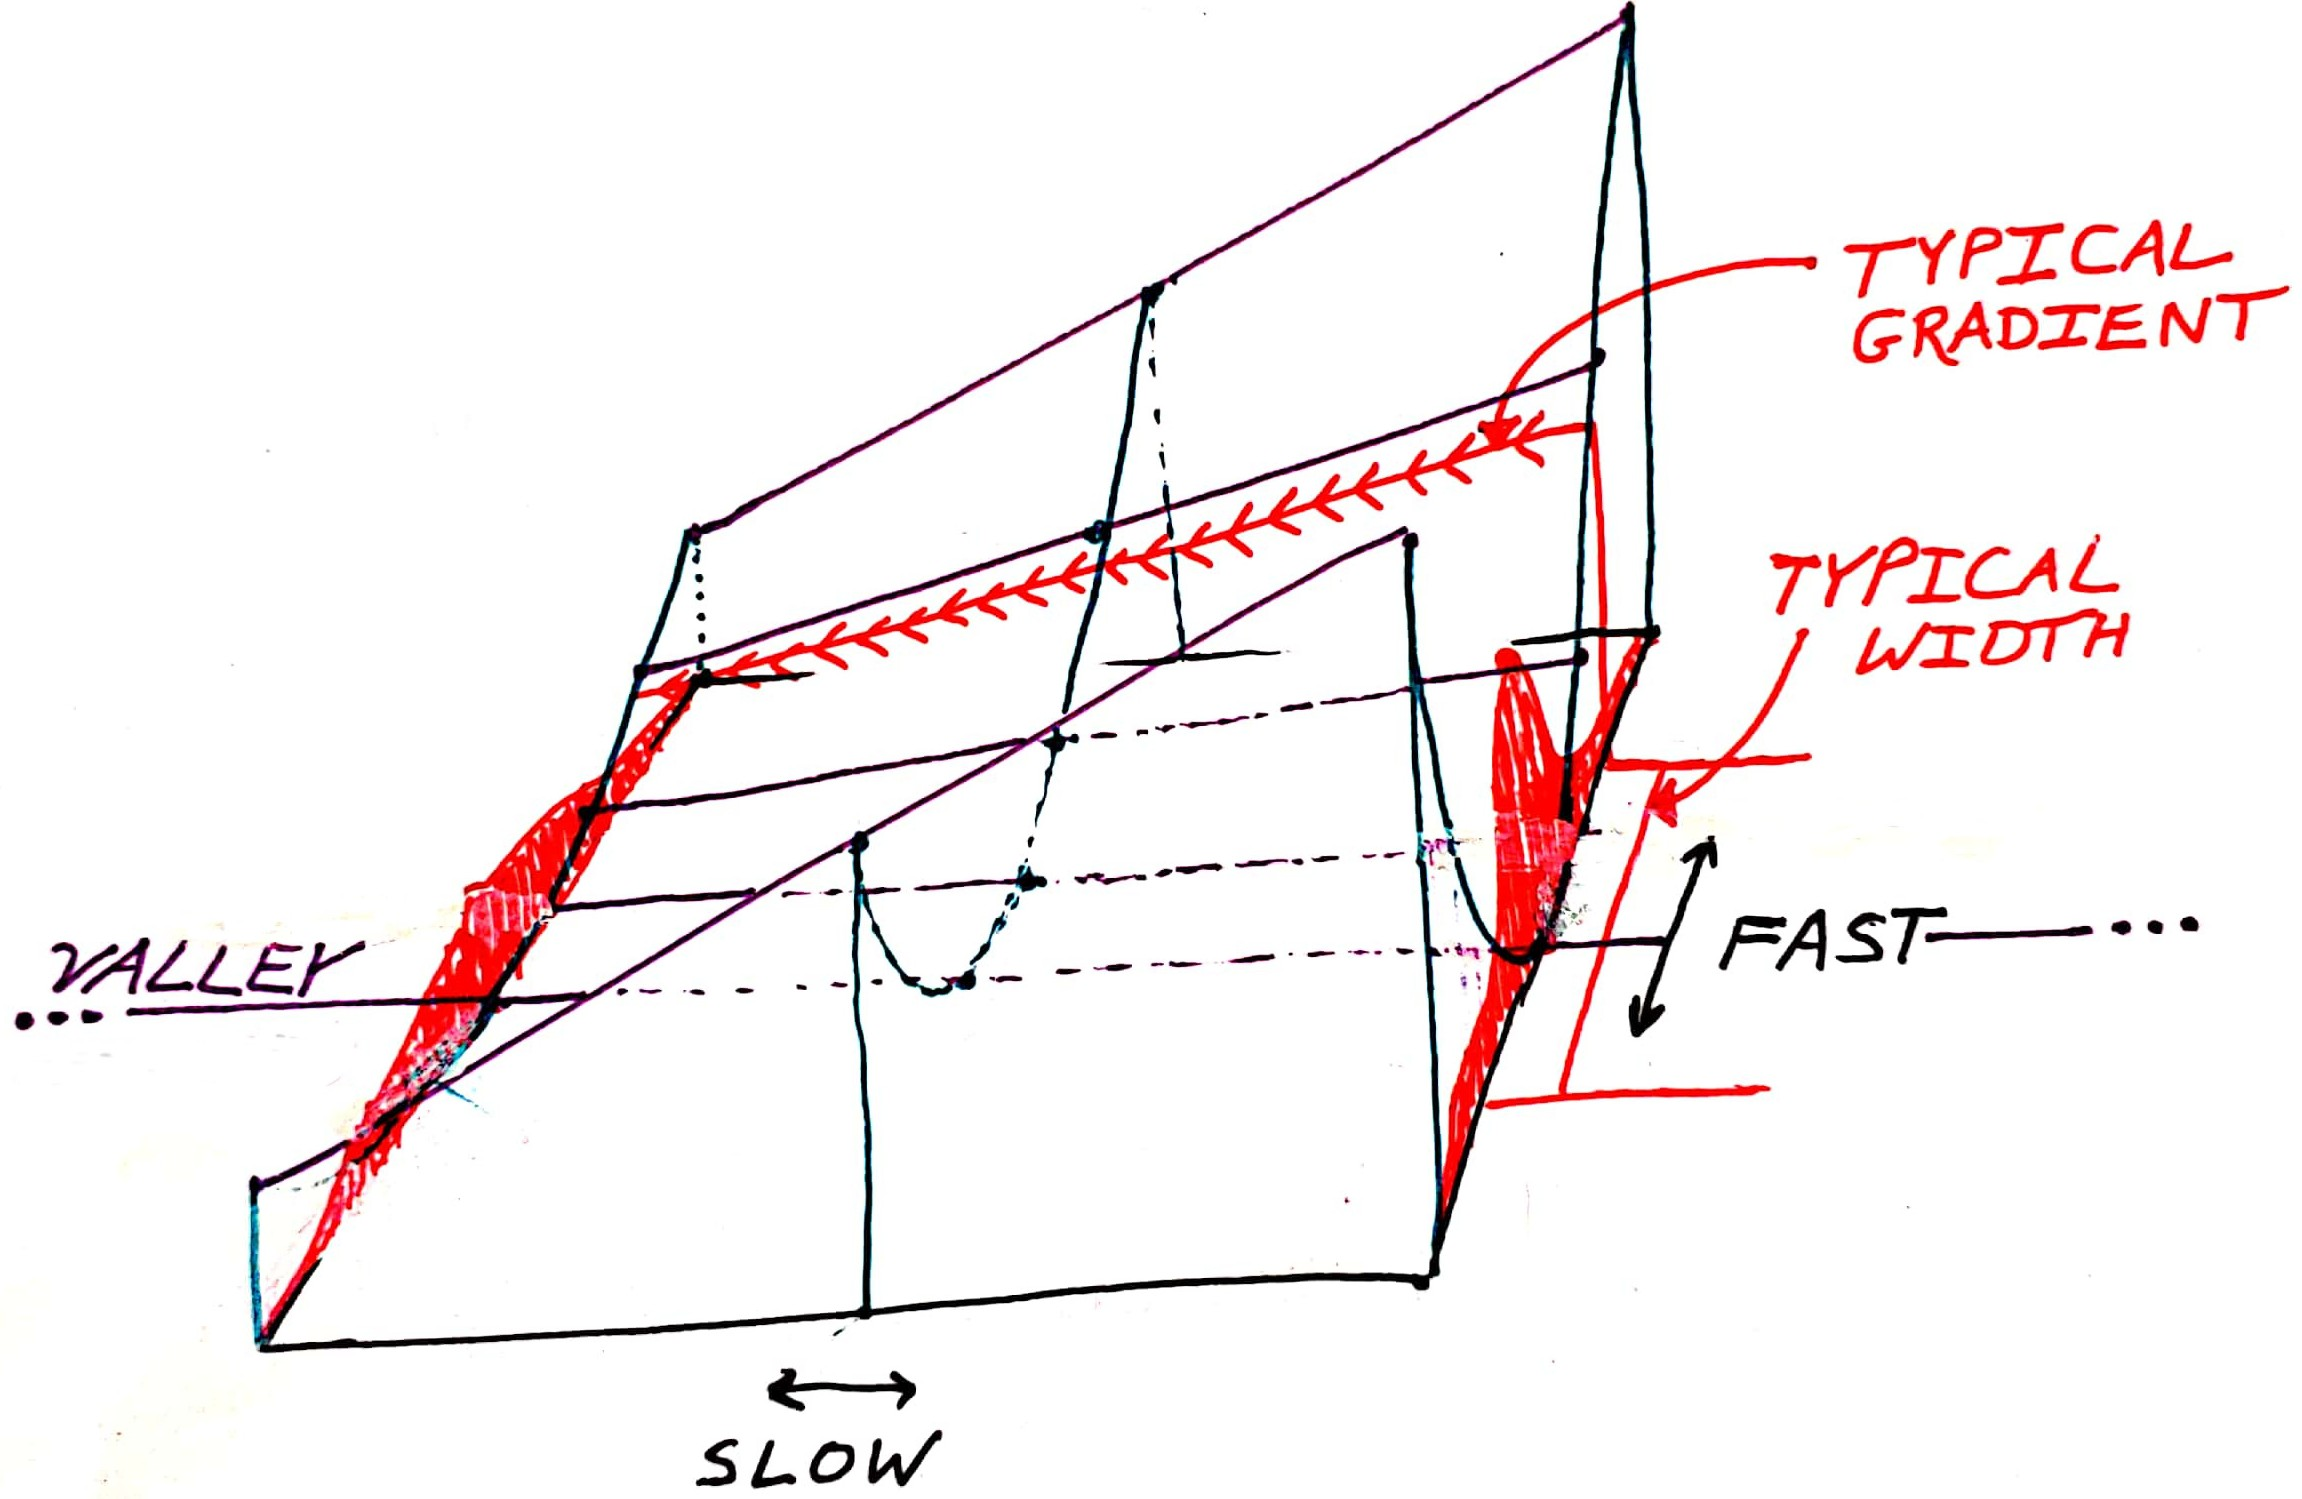
\includegraphics[height=2.2cm]{../diagrams/entropic-force-diagram}
                    \end{figure}
                \end{column}
                \begin{column}{0.55\textwidth}
                    Our main result expresses the expected test loss after $T$
                    steps of SGD as a sum over diagrams, each interpretable as
                    an interaction of weights and data.  For example, 
                    %
                    gradient noise may push $\theta_t$
                    up the valley's walls (``fast''); then 
                    $\theta_{t+1}$ will slide toward the valley's
                    flatter regions (``slow'').
                    %
                    We quantify this using the diagram $\sdia{c(01-2-3)(02-12-23)}$.
                \end{column}
                %\begin{column}{0.21\textwidth}
                %    \begin{figure}[h]
                %        \centering
                %        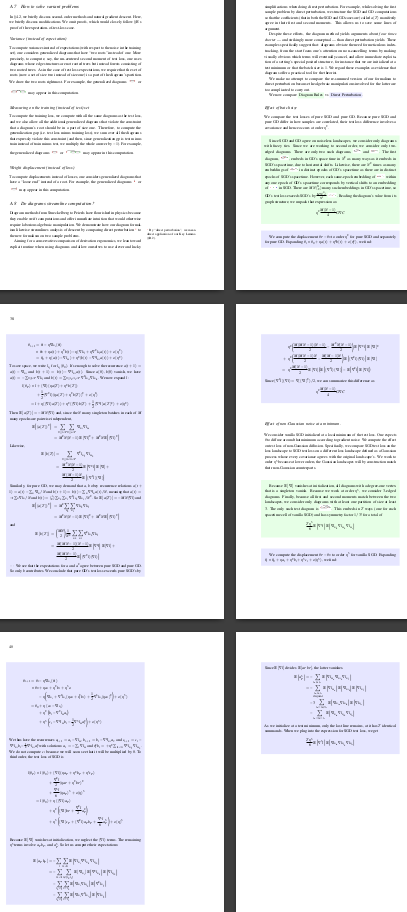
\includegraphics[height=3.2cm]{comp}
                %    \end{figure}
                %\end{column}
            \end{columns}
        }

        \frm{Diagram-based computation}{
            \envwrp{thm}{[Informal]
                SGD's expected test loss is a sum over
                weight-data interactions drawable as diagrams.  Summing the
                smallest diagrams suffices for small $\eta T$. 
            }
            \begin{columns}
                \begin{column}{0.31\textwidth}
                    \begin{figure}[h]
                        \centering
                        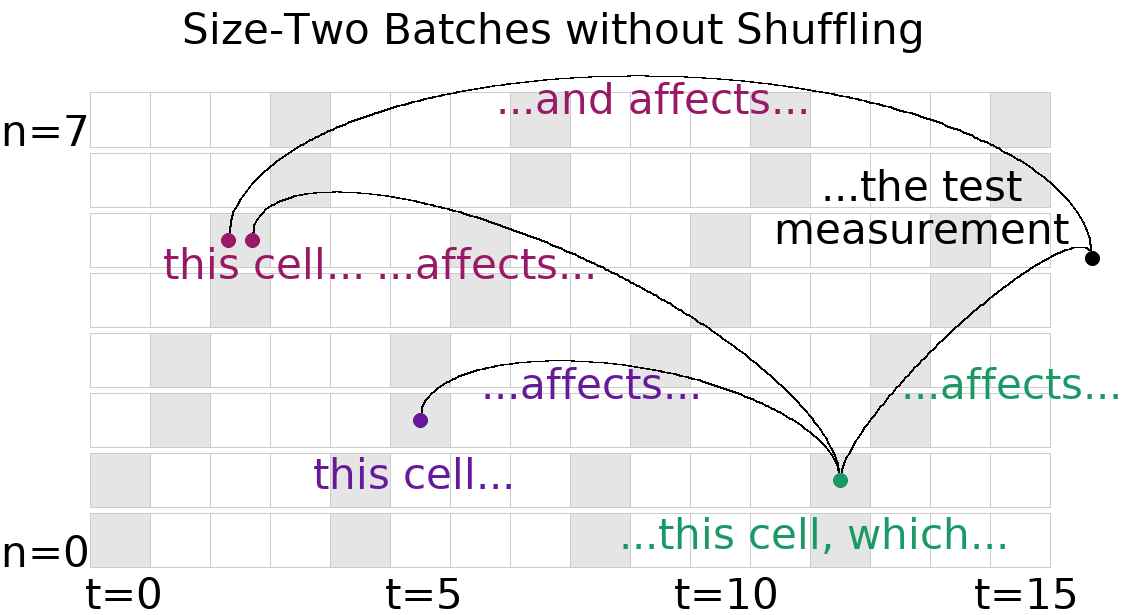
\includegraphics[height=1.8cm]{../diagrams/spacetime-f}
                    \end{figure}
                    Each diagram embeds in many ways into the grid of $(n,t)$
                    pairs s.t.\ the $t$th update involves the $n$th training
                    point.  Above:
                    an $N=8$, $T=16$ grid and the diagram
                    $\sdia{MOOc(01-2-3-4)(04-13-23-34)}$.
                \end{column}
                \begin{column}{0.67\textwidth}
                    A single diagram summarizes the effects of many related 
                    weight-data interactions (see Left).
                    \newline
                    \newline
                    Intuitively, 
                    fuzzy outlines depict correlations (noise; how
                    $\nabla l$ depends on $x$); black edges depict
                    differentiations (curvature; how $\nabla l$ depends on
                    $\theta$).
                    Thus, a diagram shows how gradient information and noise
                    flows forward in time toward the test measurement.
                    (Due to time ordering, we insist that diagrams are rooted
                    trees, drawn with root rightmost).
                \end{column}
            \end{columns}
        }
        \frm{Diagram-based computation}{
            \begin{columns}
                \begin{column}{0.83\textwidth}
                    We evaluate diagrams as follows:
                    For each \textbf{node}, write an $l_x$. 
                    For each \textbf{black edge} between two nodes,
                    differentiate the two nodes and contract them using $\eta$.
                    Group the resulting factors within expectation brackets
                    according to \textbf{fuzzy outlines}.
                    $$
                        \substack{
                            \mdia{c(0-1-2)(01-12)} \to
                        \EE[\nabla l_x] \eta
                        \EE[\nabla\nabla l_x] \eta
                        \EE[\nabla l_x]
                        \\
                        \mdia{c(01-2)(01-12)} \to
                        \EE[\nabla l_x \eta
                            \nabla\nabla l_x] \eta
                        \EE[\nabla l_x]
                    }
                    $$
                \end{column}
                \begin{column}{0.19\textwidth}
                    \begin{figure}[h]
                        \centering
                        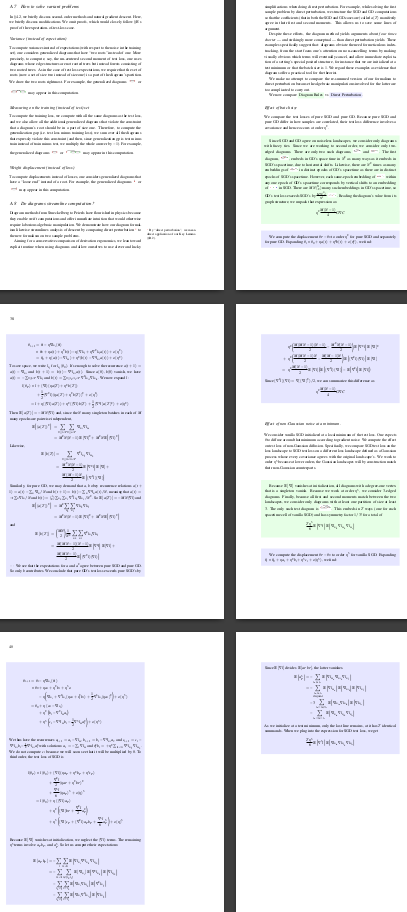
\includegraphics[height=3.0cm]{comp}
                    \end{figure}
                \end{column}
            \end{columns}
                    \envwrp{exm}{[\emph{Does skewed noise affect test loss?}]
                        To leading order, the test loss due to skewed noise is
                            $
                               \sdia{c(012-3)(03-13-23)}
                            $,
                        which for large $T$ and isotropic $H$ evaluates to
                            $
                               - \frac{\eta^3}{3!}
                                 \frac{{\color{moor}S}_{\mu\nu\lambda}
                                       {\color{moog}J}_{\mu\nu\lambda}}
                                      {3 \|\eta H\|_2}
                            $.
                        Here, 
                        we used the skewness and jerk
                        {\footnotesize
                        $$
                            S=\EE (\nb\lx - G)^3= \sdia{MOOc(012)(0-1-2)}
                            ~~~~~
                            J=\EE (\nb\nb\nb\lx)=\sdia{MOO(0)(0-0-0)}
                        $$
                        }
                        and $G,H$ are the expected gradient and hessian.
                    }
        }

        \frm{Problem setup}{
            %\begin{columns}
                %\begin{column}{0.75\textwidth}
                    Fix a data distribution $\Dd$, a manifold $\Hh$ of weights, and
                    a loss landscape $l:|\Dd|\to\Hh\to\RR$, considered as a random
                    function.  For an initialization $\theta_0\in\Hh$ and a
                    sequence $x_t\sim \Dd: 0\leq t<T$, we consider the iteration
                    $$
                        \theta_{t+1} = \theta_t - \eta \nabla l_{x_t} (\theta_t)  
                    $$
                    We use such \textbf{stochastic gradient descent} in learning, as an
                    approximate optimizer.  Compare to $T\to\infty$ limits: fixing
                    $\eta T$, we recover \textbf{ODE}; fixing $\eta \sqrt{T}$, we recover
                    \textbf{SDE}.  More generally, if $\Ss = (x_n:0\leq n<N) \sim
                    \Dd^N$ and we update with $l_{\Bb_t} = \sum_{n\in
                    \Bb_t}l_{x_n}/|\Bb_t|$, then \textbf{GD} is SGD with $\Bb = \Ss$. 
                %\end{column}
            %\end{columns}
            %
            \envwrp{qst}{
                How does SGD's dynamics on a curved and noisy landscape affect
                optimization and 
                generalization?
                How does SGD differ from GD, SDE?
            }
            We wish to express
                $\EE_{\Ss}l_x$ and 
                $\EE_{\Dd}l_x-\EE_{\Ss}l_x$
            (at $\theta_T$) in terms of $l$'s statistics.
        }


    \section{Results}

        \frm{Theory}{
            \begin{columns}
                \begin{column}{0.59\textwidth}
                    The Theorem below expresses SGD's test loss as a sum over
                    diagrams.  A diagram with $d$ edges scales as $O(\eta^d)$,
                    so the following is a series in $\eta$.  We later truncate
                    the series to small $d$, focusing on few-edged diagrams.
                    \begin{thm}[Re-summation] \label{thm:resum}
                        For $|\Bb|=1$ and any $T$: for $\eta$ small enough, SGD
                        has expected test loss
                        \begin{equation*} \label{eq:resum}
                            \sum_{\substack{D~\text{an irreduc-} \\ \text{-ible diagram}}}
                            ~
                            \sum_{\substack{f~\text{an embed-} \\ \text{-ding of}~D}}
                            ~
                            \frac{(-1)^{|\text{edges}(D)|}}{|\text{Aut}_f(D)|}
                            \,
                            {\text{rvalue}_f}(D)
                        \end{equation*}
                    \end{thm}
                    We may approximate sums by integrals and $(I-\eta H)^t$ by
                    $\exp(- \eta H t)$, reducing to a routine integration of
                    exponentials with error factor $1 + o(\eta)$.
                \end{column}
                \begin{column}{0.39\textwidth}
                    \begin{thm}[Convergence]
                        If $\theta_\star$ is a non-degenerate local minimum of
                        $l$ (i.e.\ $G(\theta_\star)=0$ and $H(\theta_\star) >
                        0$), then for SGD initialized sufficiently close to
                        $\theta_\star$, the $d$th-order truncation of Theorem
                        \ref{thm:resum} converges as $T\to \infty$.
                    \end{thm}
                    The above $T\to \infty$ limit might not measure any
                    well-defined limit of SGD, since the limit might not
                    commute with the infinite sum.  We see no such pathologies
                    in practice, so we freely speak of ``SGD in the large-$T$
                    limit.''
                \end{column}
            \end{columns}
        }

        \frm{High-$C$ regions repel SGD}{
            \begin{figure}[h]
                \centering
                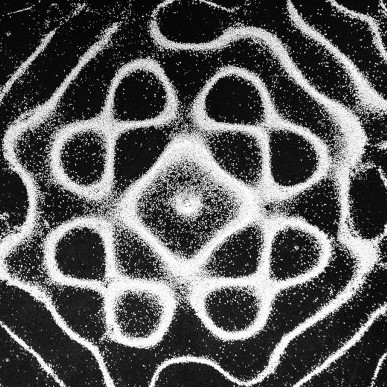
\includegraphics[height=2cm]{../plots/chladni}
                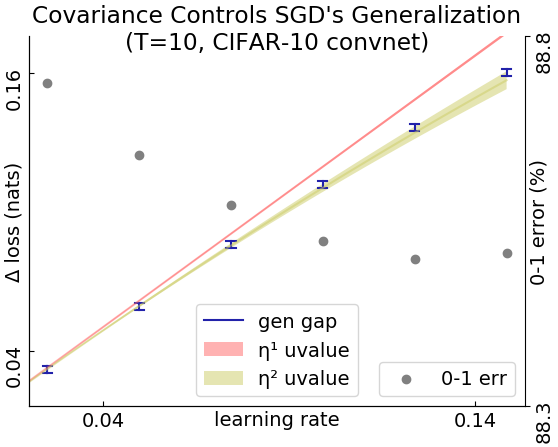
\includegraphics[height=2cm]{../plots/neurips-gen-cifar-lenet}
                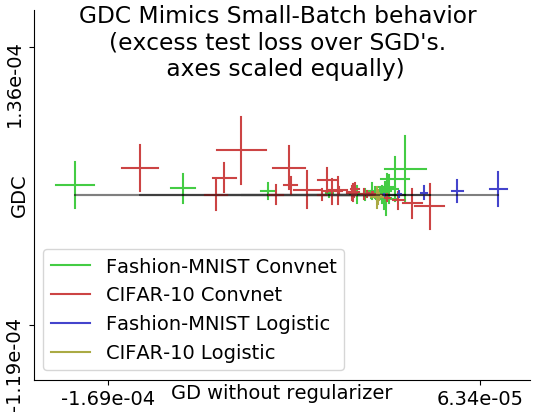
\includegraphics[height=2cm]{../plots/new-big-bm-new}          
                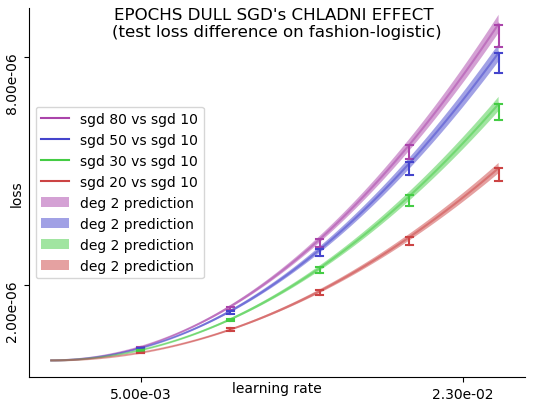
\includegraphics[height=2cm]{../plots/multi-fashion-logistic-0}
            \end{figure}
            %Physical intuition %(\S\ref{appendix:interpret-diagrams})
            %suggests
            %that noise repels SGD.  
            If two neighboring regions
            of weight space have high and low levels of gradient noise,
            respectively, then we expect the rate at which $\theta$ jumps from
            the former to the latter to exceed the opposite rate.  Hence,
            net movement toward regions of small $C$! 
            More precisely, the drift is in the
            direction of $-\nabla C$.  The effect is strongest when gradient
            noise is not averaged out by large batch sizes, but we may counter
            this effect via an artificial loss term:\footnote{
                We call the resulting optimization method \textbf{GDC}.
            }
            \begin{cor}[$\sdia{c(01-2)(01-12)}$] \label{cor:batch}
                SGD avoids high-$C$ regions more than GD:
                $
                    l_{C}
                        \triangleq
                    \frac{N-1}{4 N}
                    \nabla^\mu C^{\nu}_{\nu}
                        =
                    \EE({\theta_{GD} - \theta_{SGD}})^\mu - o(\eta^2)
                $.
                If $\hat{l_c}$ is a smooth unbiased estimator of $l_c$, then GD
                on $l + \hat{l_c}$ has an expected test loss that agrees with
                SGD's to order $\eta^2$.  
            \end{cor}
        }

        \frm{SGD prefers minima flat with respect to $C$}{
            \begin{figure}[h]
                \centering
                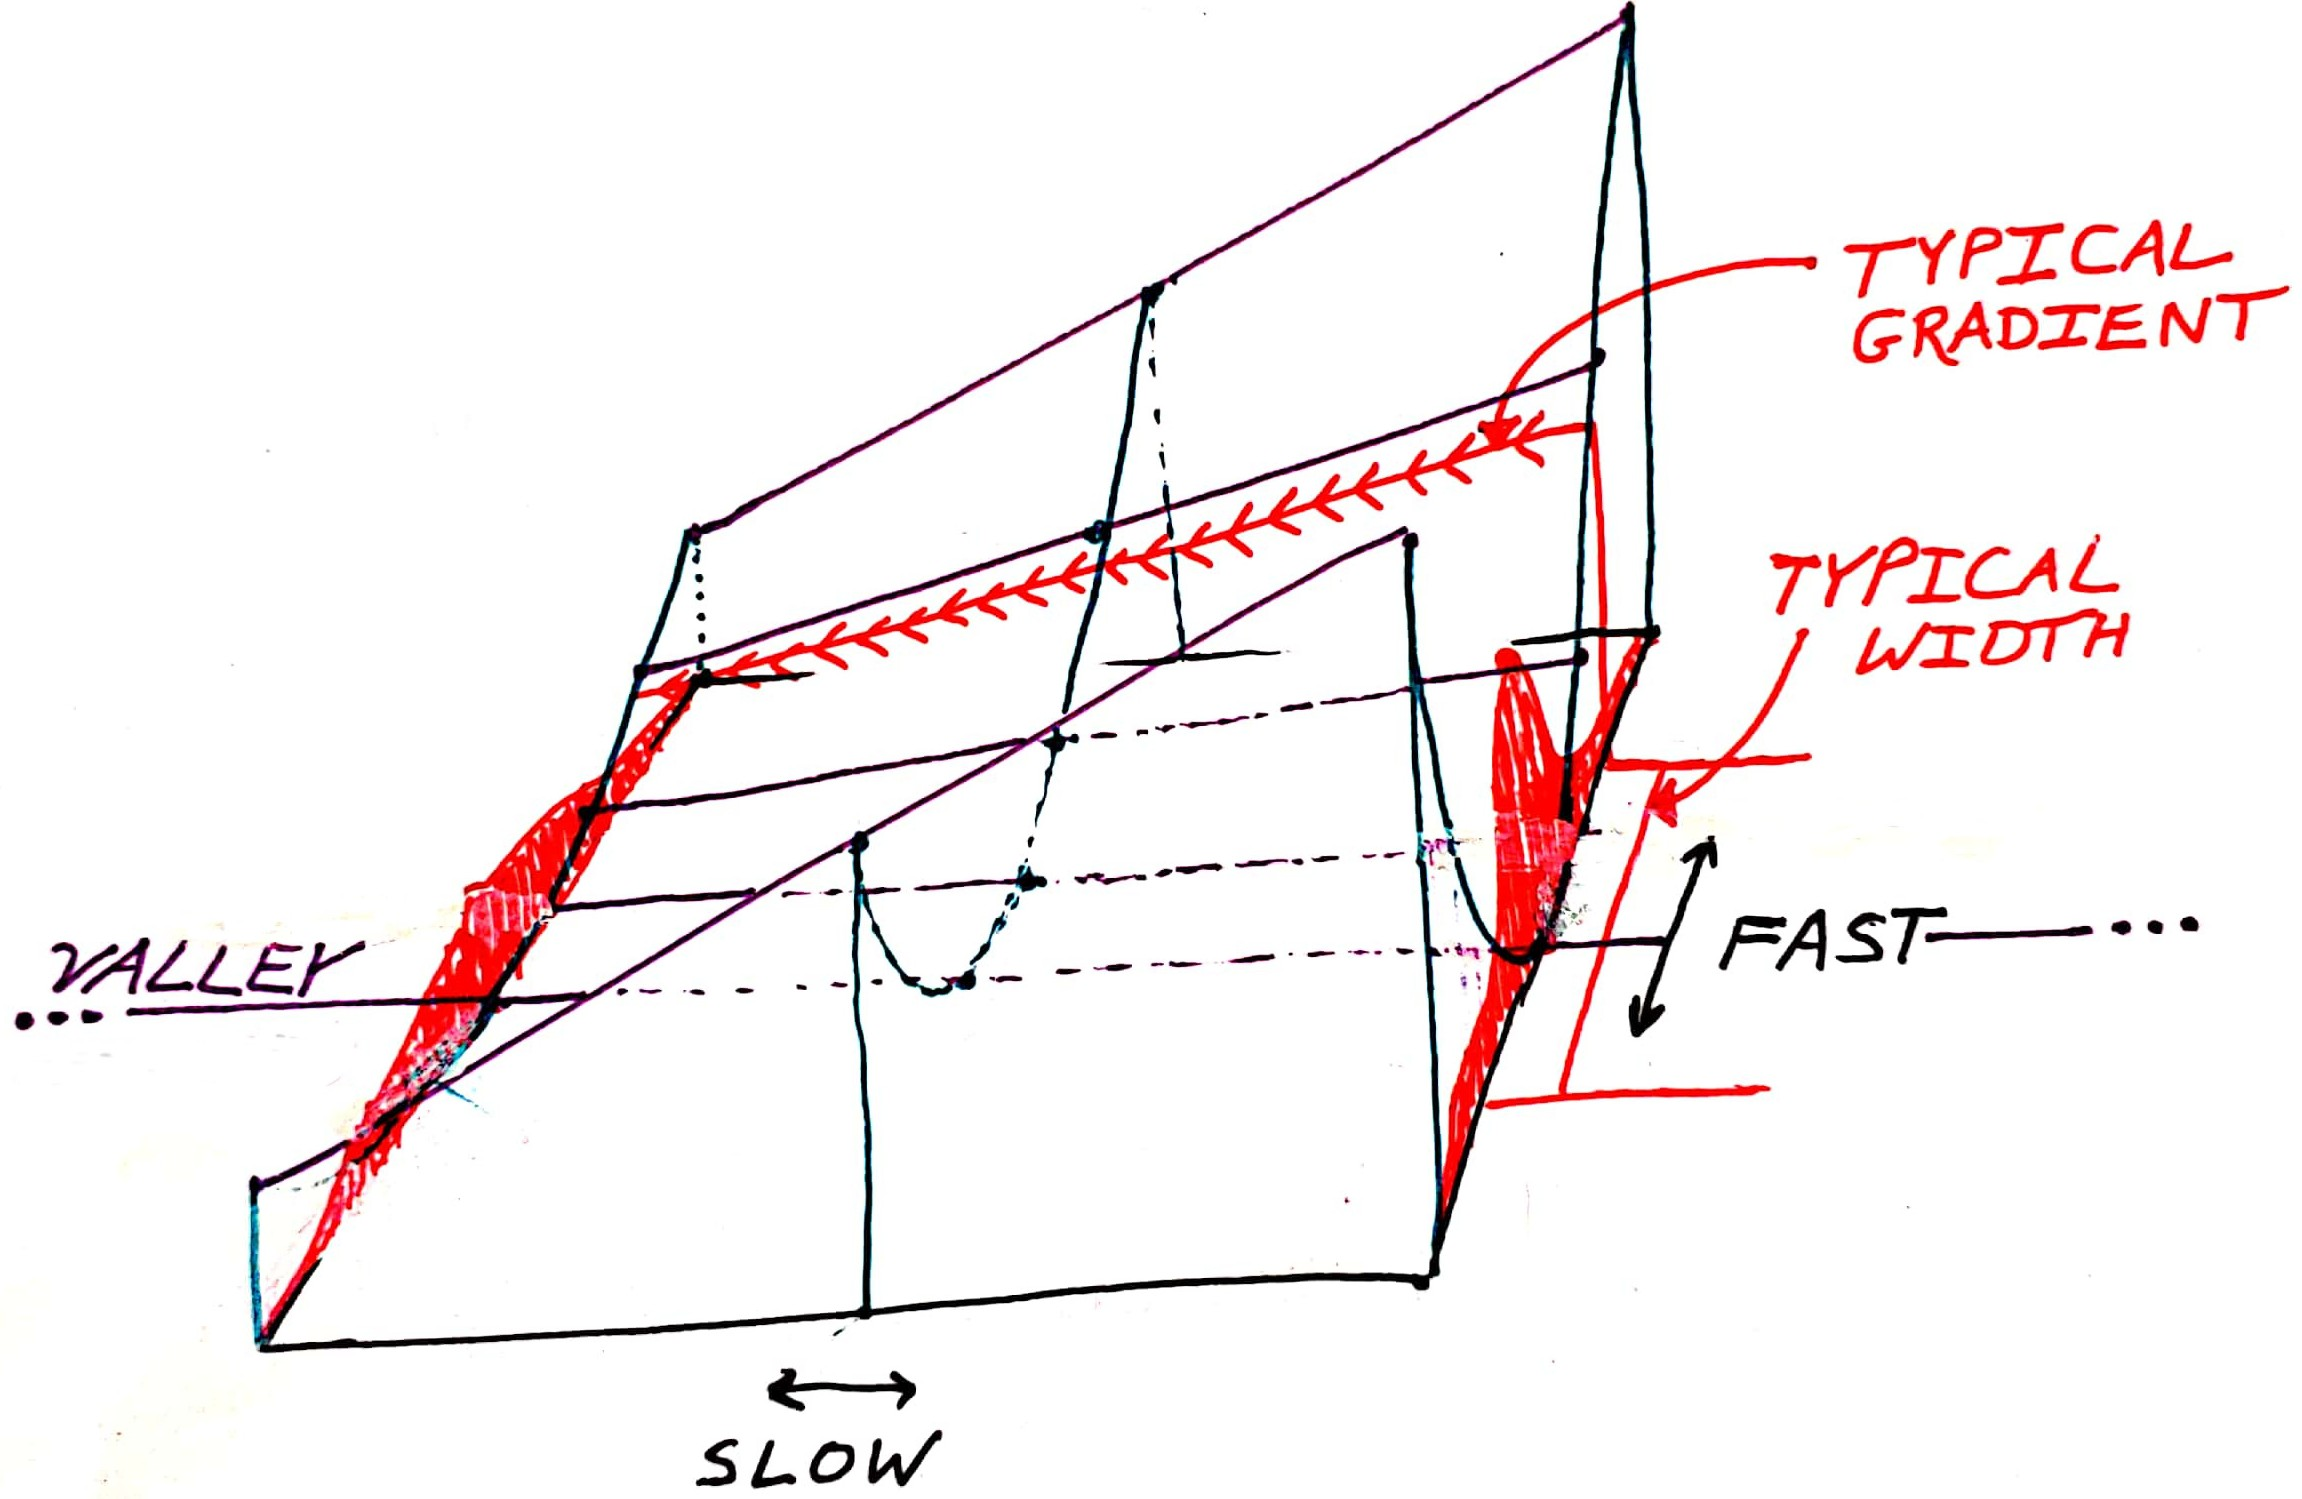
\includegraphics[height=2.2cm]{../diagrams/entropic-force-diagram}
                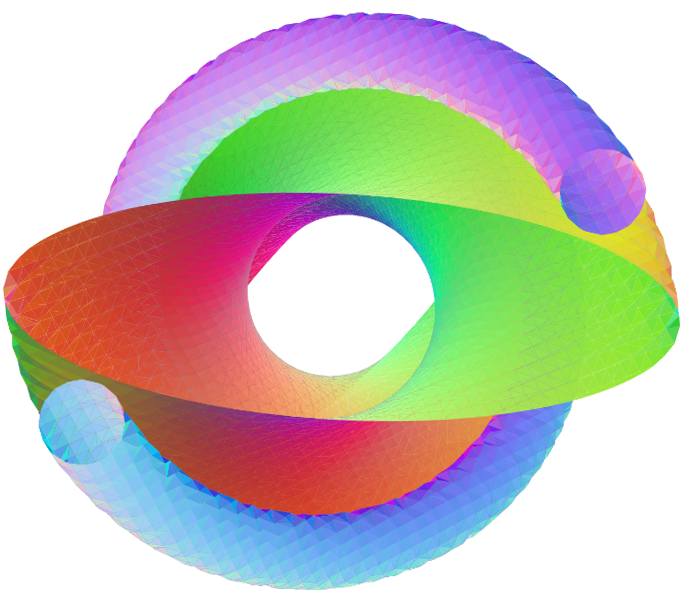
\includegraphics[height=1.8cm]{../plots/from-above}
                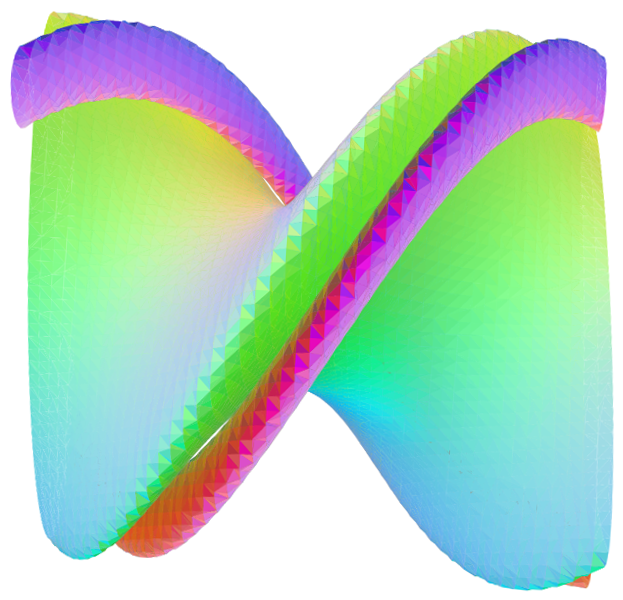
\includegraphics[height=1.8cm]{../plots/from-side}
                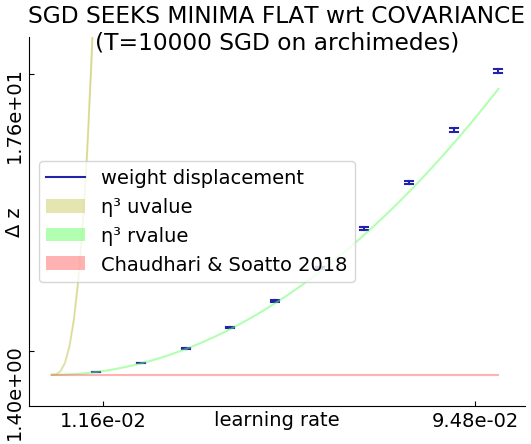
\includegraphics[height=2.2cm]{../plots/neurips-thermo-linear-screw}
            \end{figure}
            \begin{columns}
                \begin{column}{0.59\textwidth}
                    Gradient noise may push $\theta_t$
                    up the valley's walls (``fast''); then 
                    $\theta_{t+1}$ will slide toward the valley's
                    flatter regions (``slow'').
                    \begin{cor}[Computed from $\sdia{c(01-2-3)(02-12-23)}$]
                        \label{cor:entropic}
                        Run SGD for $T \gg 1/\eta H$ from a non-degenerate test
                        minimum.  Written in an eigenbasis of $\eta H$, $\theta$ has an
                        expected displacement of
                        $$
                            - \frac{\eta^3}{2}
                            \sum_{\mu\nu}
                                C_{\mu\nu}
                                \frac{1}{\eta (H_{\mu\mu} + H_{\nu\nu})}
                                J_{\mu\nu\lambda}
                                \frac{1}{H_{\lambda\lambda}}
                            + o(\eta^2)
                        $$
                    \end{cor}
                \end{column}
                \begin{column}{0.39\textwidth}
                    %
                    $CH/2+o(C)$ is the increase upon
                    convolving $l$ with a $C$-shaped Gaussian:
                    SGD descends on a $C$-smoothed landscape.
                    %
                    %\newline
                    %\newline
                    %
                    This landscape changes as $C$ does, so
                    SGD's velocity field generically has
                    \emph{curl}.  Indeed, 
                    while $\nabla(CH)$ is a total
                    derivative, $C\nabla H$ is not.  
                    %
                    Contrast to \citet{we19b}'s assumptions constant $C$
                    analysis.
                    %
                    %By avoiding \citet{we19b}'s assumptions of constant $C$,
                    %we find that SGD pursues
                    %directions, not locations, and it may cycle forever.
                \end{column}
            \end{columns}
        }

        \frm{Both flat and sharp minima overfit less}{
            \begin{figure}[h]
                \centering
                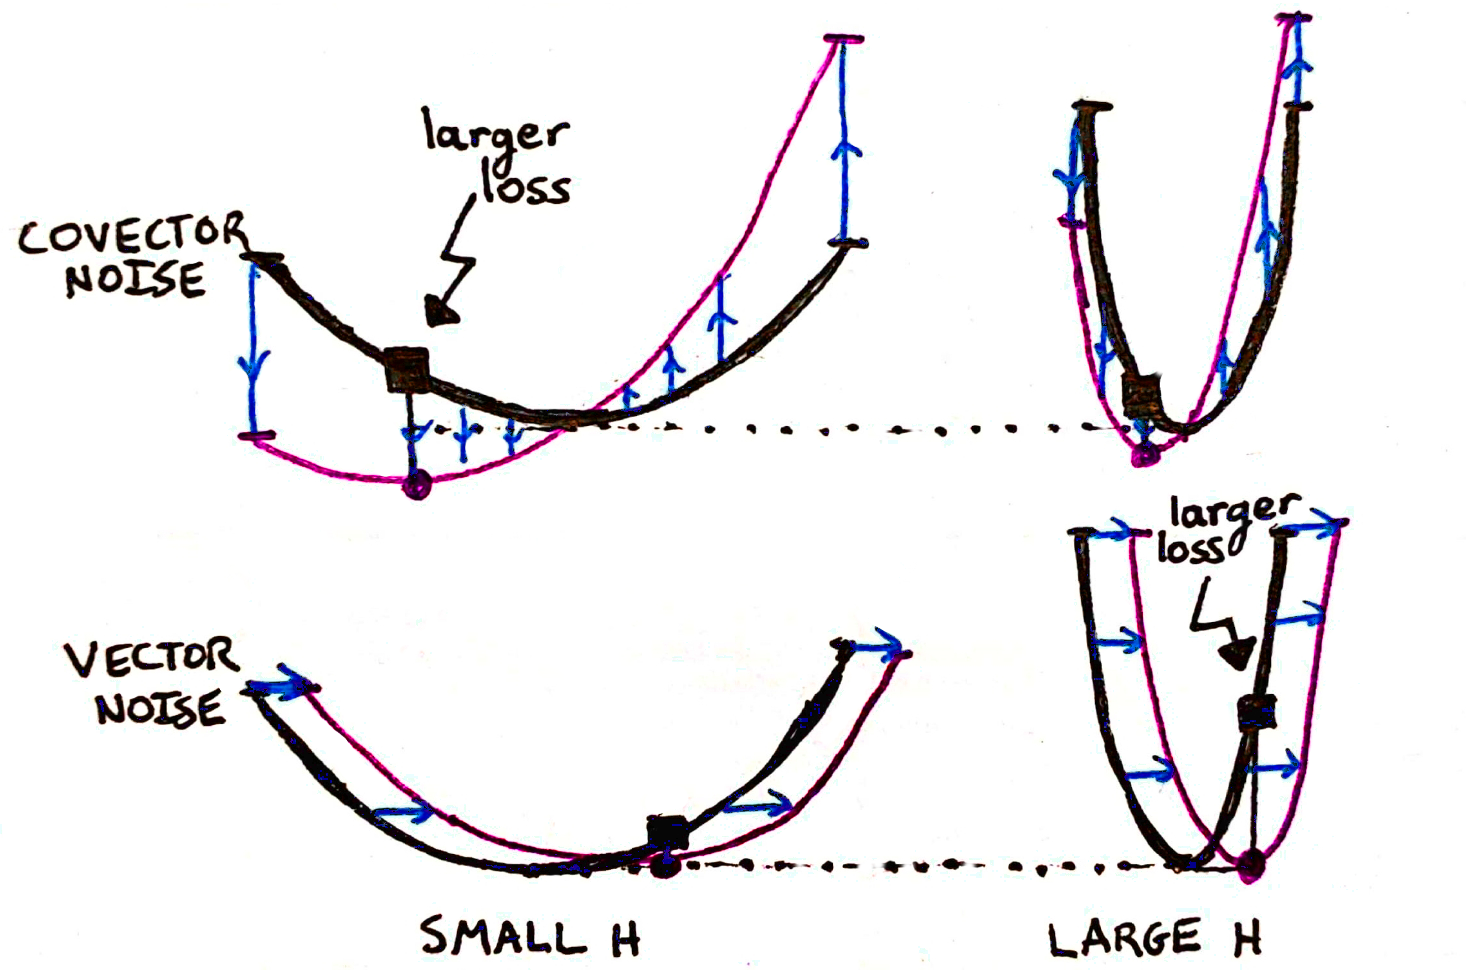
\includegraphics[height=2.5cm]{../diagrams/sharp}
                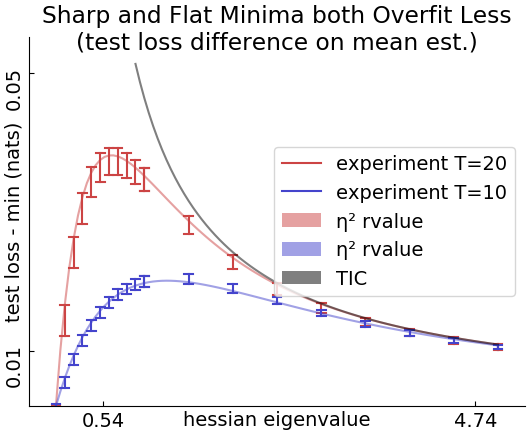
\includegraphics[height=2.5cm]{../plots/neurips-tak}
                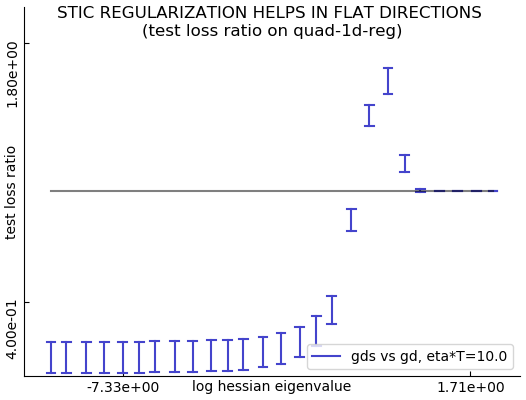
\includegraphics[height=2.5cm]{../plots/tak-reg}
            \end{figure}
            %
            It is obvious that SGD overfits less near \textbf{sharp} minima.
            Prior work empirically supports this claim;
            after all, $l_2$ regularization acts by increasing the Hessian.
            \newline
            \newline
            It is also obvious that SGD overfits less near \textbf{flat}
            minima.  Prior work empirically supports this claim; after all,
            flat minima are stable as the weight changes.
            \newline
            \newline
            More balanced view:  Sharp minima are robust
            to slight changes in the average \emph{gradient} and flat minima
            are robust to slight
            \emph{displacements} in weight space.
            %
            As we take $T\to \infty$:
            overfitting $\to \text{TIC} = C/2NH$.  Prior works
            such as \citet{di18} use TIC to estimate overfitting but
            require arbitrary cutoffs for
            singular $H$.  Counter
            to intuition!  Our theory
            shows that the implicit regularization of
            finite-$T$ descent tames these singularities: the
            overfitting formula tends to $0$ as $H$ shrinks.
        }

    \section{Conclusion}
        \frm{Contributions}{
            We presented a diagram-based method for studying stochastic
            optimization on short timescales or near minima.  The corollaries
            offer insight
            into SGD's success in training deep networks: SGD avoids curvature
            and noise, and curvature and noise control generalization.
            \newline\newline Analyzing $\sdia{c(01-2)(02-12)}$, we proved that
            \textbf{flat and sharp minima both overfit less} than medium
            minima.  Intuitively, flat minima are robust to vector noise, sharp
            minima are robust to covector noise, and medium minima robust to
            neither.  We thus proposed a regularizer enabling gradient-based
            hyperparameter tuning.
            %
            Inspecting $\sdia{c(01-2-3)(02-12-23)}$, we extended \citet{we19b}
            to nonconstant, nonisotropic covariance to reveal that \textbf{SGD
            descends on a landscape smoothed by the current covariance $C$}.
            As $C$ evolves, the smoothed landscape evolves, resulting in
            non-conservative dynamics.
            %
            Examining $\sdia{c(01-2)(01-12)}$, we showed that \textbf{GD may
            emulate SGD}, as conjectured by \citet{ro18}.  This is significant
            because, while small batch sizes can lead to better
            generalization,\cite{bo91} modern infrastructure increasingly
            rewards large batch sizes.\cite{go18} 
        }

        \frm{Related work; limitations}{
            SGD-trained networks generalize despite their ability to shatter
            large sets \citep{zh17}, so generalization must arise from the
            aptness-to-data of not only architecture but also
            \textbf{optimization} \citep{ne17b}.
            %
            \newline \newline
            %
            Approaches via \textbf{stochastic differential equations} assume
            uncorrelated, Gaussian noise in continuous time \citep{ch18, li17};
            per \citet{ya19a}, they cannot cannot treat SGD noise correctly.
            %
            Prior \textbf{perturbative approaches} were limited to specific
            neural architectures \citep{dy19} or to computing Gaussian
            statistics over $T=2$ \citep{ro18}. 
            %
            We do not assume \textbf{information-geometric} relations between
            $C$ and $H$, so we may model VAEs. 
            %
            \newline \newline
            %
            Our predictions depend only on loss data near $\theta_0$, so they
            only apply for long times (large $\eta T$) near an isolated minimum
            or for short times (small $\eta T$) in general.  
            %
            Meteorologists understand how warm and cold fronts interact
            \textbf{despite long-term intractability} [\S C.1]; we quantify
            curvature's and noise's counter-intuitive effects in each
            short-term interval of SGD.
        }

        \frm{Future directions: Lagrangians and curved backgrounds}{
            Our diagrams invite exploration of Lagrangian formalisms and curved
            backgrounds:
            \begin{qst}
                Does some least-action principle govern SGD; if not, what is an
                essential obstacle to this characterization?
            \end{qst}
            %Lagrange's least-action formalism intimately intertwines with the
            %diagrams of physics.  Together, they afford a modular framework for
            %introducing new interactions as new terms or diagram nodes.
            %In fact,
            Some \emph{higher-order} methods --- such as the
            $H$-based update
            $
                \theta \leftarrow
                \theta -
                (\eta^{-1} + \lambda \nabla \nabla l_t(\theta))^{-1}
                \nabla l_t(\theta)
            $
            parameterized by small $\eta, \lambda$ --- admit diagrammatic analysis
            when we represent the $\lambda$ term as a second type of node.
            %Though diagrams suffice for computation, it is Lagrangians that most
            %deeply illuminate scaling and conservation laws.
            \newline
            \newline
            Our work assumes a flat metric $\eta^{\mu\nu}$, but it might
            generalize to curved spaces.\footnote{
                One may represent the affine connection as a node, thus giving
                rise to non-tensorial and hence gauge-dependent diagrams.
            }
            %Such curvature finds concrete application in the \emph{learning on
            %manifolds} paradigm,\cite{ab07, zh16} notably specialized to
            %\citet{am98}'s \emph{natural gradient descent} and \citet{ni17}'s
            %\emph{hyperbolic embeddings}.
            Prior work focuses on
            \emph{optimization} on curved weight spaces, in machine learning we
            also wish to analyze \emph{generalization}.
            %
            %Starting with the intuition that ``smaller'' hypothesis classes
            %generalize better and that curvature controls the volume of small
            %neighborhoods, we conjecture that sectional curvature regularizes
            %learning:
            \begin{conj}[Sectional curvature regularizes]
                If $\eta(\tau)$ is a Riemann metric on weight space, smoothly
                parameterized by $\tau$, and if the sectional curvature through
                every $2$-form at $\theta_0$ increases as $\tau$ grows, then
                the generalization\ gap attained by fixed-$T$ SGD with learning rate $c
                \eta(\tau)$ (when initialized from $\theta_0$) decreases as $\tau$
                grows, for all sufficiently small $c>0$.
            \end{conj}
            %We are optimistic our formalism may resolve conjectures such as above.
        }
        %\frm{Bird's eye view}{
        %    Lorem ipsum dolor sit amet, consectetur adipisicing elit, sed
        %    do eiusmod tempor incididunt ut labore et dolore magna aliqua.
        %}

        \frm{Bibliography}{
            \bibliographystyle{plainnat}
            \bibliography{perturb}
        }

\end{document}

        %    \begin{columns}
        %        \begin{column}{0.59\textwidth}
        %        \end{column}
        %        \begin{column}{0.59\textwidth}
        %        \end{column}
        %    \end{columns}

